\documentclass{beamer}
\usepackage[utf8]{inputenc}
\usepackage{hyperref}
\usepackage{listings}

\lstdefinestyle{saneCode}{
    belowcaptionskip=1\baselineskip,
    breaklines=true,
    frame=none,
    numbers=none,
    basicstyle=\scriptsize\ttfamily,
    % keywordstyle=\bfseries\color{green!40!black},
    % commentstyle=\itshape\color{purple!40!black},
    % identifierstyle=\color{blue},
    backgroundcolor=\color{gray!10!white},
}

\usetheme{Singapore}
\usecolortheme{default}

\title[Academic Websites with Hugo]{Building an Academic Website in 60 Minutes}
\subtitle{(with the help of Hugo)}
\author[Thompson, VanIwaarden]{
  Thompson, Jonathan\\
  \and
  VanIwaarden, River\\
}

\institute[UCCS]{University of Colorado at Colorado Springs}

\date[UCCS 2022]
{AMS Graduate Chapter Website Workshop \\ May 02, 2022}

% \logo{\includegraphics[height=1cm]{overleaf-logo}}

\begin{document}

% Title Page
\frame{\titlepage}

% Presentation Content
\begin{frame}
    \frametitle{Prerequisites}

    Here's what we'll need for this workshop:
    \bigskip

    \begin{enumerate}[<+->]
        \setlength\itemsep{3em}
        \item Git: \url{https://git-scm.com/downloads}
        \begin{itemize}
            \item Why? Git is a version control system used to manage any kind of source code 
                  (C, MATLAB, LaTeX, etc.).
        \end{itemize}

        \item That's it!
    \end{enumerate} 
\end{frame}
\begin{frame}
    \frametitle{Background}

    What comprises a website?
    \bigskip

    \begin{enumerate}[<+->]
        \setlength\itemsep{2em}
        \item HTML: \textbf{H}yper\textbf{T}ext \textbf{M}arkup \textbf{L}anguage
        \begin{itemize}
            \item HTML describes the \textbf{content} of a webpage.
        \end{itemize}
        \item CSS: \textbf{C}ascading \textbf{S}tyle \textbf{S}heets
        \begin{itemize}
            \item CSS describes the \textbf{style} of a webpage.
        \end{itemize}
        \item JavaScript
        \begin{itemize}
            \item JavaScript describes \textbf{how elements interact} on a webpage.
        \end{itemize}
    \end{enumerate}

    \bigskip
    \onslide<+->{Building websites from scratch takes a lot of work!}
\end{frame}
\begin{frame}
    \frametitle{Introduction to Hugo}

    Building a website from scratch is a bit like building a PDF document from scratch:

    \bigskip

    \begin{itemize}[<+->]
        \setlength\itemsep{2em}
        \item Doing so provides the most flexibility, but is also excessive for most purposes.
        \item There exist tools to create websites visually, but these tools tend to be specialized and difficult to
              collaborate with.
        \item For our purposes, we often care more about content than we do about customization.
    \end{itemize}

    \bigskip
    \onslide<+->{This is where Hugo comes in!}
\end{frame}
\begin{frame}
    \frametitle{Markdown}

    Markdown is a simple markup language for creating \textbf{formatted text} designed to be easily readable in
    its source code form.
    \medskip

    \pause
    \begin{columns}
        \begin{column}[T]{.45\textwidth}
            Hugo takes Markdown...\ \\
            \smallskip
            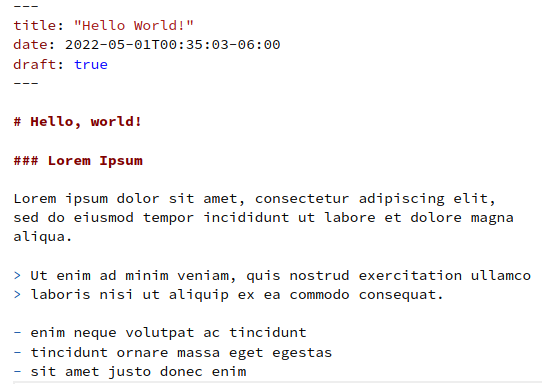
\includegraphics[width=\textwidth]{images/markdown.png}
        \end{column}
        \pause
        \begin{column}[c]{.1\textwidth}
            $$ \to $$
        \end{column}
        \begin{column}[T]{.45\textwidth}
            ...and turns it into a webpage:\ \\
            \smallskip
            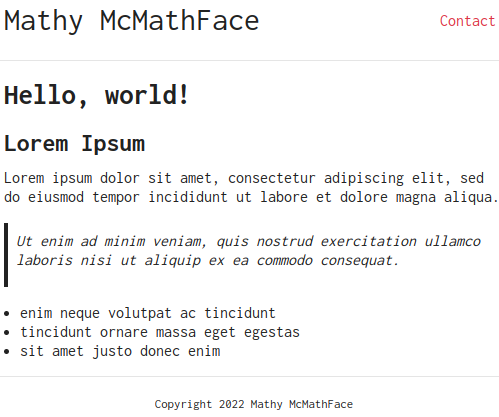
\includegraphics[width=\textwidth]{images/rendered_markdown.png}
        \end{column}
    \end{columns}

    \pause
    \vfill

    In many ways, Hugo does for webpages what \LaTeX \: does for documents.
    
\end{frame}
\begin{frame}
    \frametitle{Getting Started}

    First, we need to open a command line. The command line (also known as a terminal or console) is
    an invaluable tool for executing text commands on a computer.
    \medskip
    
    \begin{columns}
        \begin{column}{.45\textwidth}
            \begin{block}{Windows}
                From the Start Menu, open the \texttt{Git Bash} application:
                
\includegraphics[width=\textwidth]{images/windows_gitbash.png}
            \end{block}
        \end{column}

        \begin{column}{.45\textwidth}
            \begin{block}{MacOS}
                Open the \texttt{Terminal} application from Launchpad:
                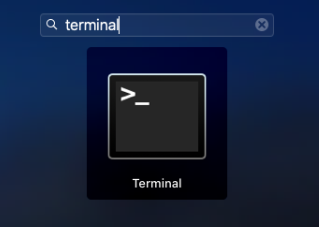
\includegraphics[width=\textwidth]{images/macos_terminal.png}
            \end{block}
        \end{column}
    \end{columns}
\end{frame}
\begin{frame}[fragile]
    \frametitle{Getting Started}

    Now we'll change directories (\texttt{cd}) to the \texttt{Desktop} folder.  Type the following into your terminal
    (\textbf{without} the "\$" character\footnote{
        It is customary to add this character in technical documentation to indicate that the proceeding
        command is to be entered into a terminal.
    }), and then hit the \texttt{[Enter]} key:
   
    \bigskip
    
    \begin{lstlisting}[style=saneCode,gobble=8]
        $ cd Desktop
    \end{lstlisting}

    \vfill
    Next, we'll use Git to clone (download) all the necessary code for this project. Type the following command into
    your terminal, and then hit the \texttt{[Enter]} key:

    \bigskip

    \begin{lstlisting}[style=saneCode,gobble=8]
        $ git clone https://github.com/uccs-ams/website-workshop.git --recurse
    \end{lstlisting}


\end{frame}
\begin{frame}[fragile]
    \frametitle{Getting Started}

    Let's change directories again to the newly-created \texttt{website-workshop} folder:
   
    \bigskip
    
    \begin{lstlisting}[style=saneCode,gobble=8]
        $ cd website-workshop
    \end{lstlisting}

    \vfill

    The next command we need to run depends on our operating system. We're going to check out slightly different
    versions of the code to account for operating system differences:

    \medskip

    \begin{block}{Windows}
    \begin{lstlisting}[style=saneCode,gobble=8]
        $ git checkout windows
    \end{lstlisting}
    \end{block}
    
    \begin{block}{MacOS}
    \begin{lstlisting}[style=saneCode,gobble=8]
        $ git checkout macos
    \end{lstlisting}
    \end{block}

    \begin{block}{MacOS [M1]}
    \begin{lstlisting}[style=saneCode,gobble=8]
        $ git checkout macos-arm64
    \end{lstlisting}
    \end{block}

\end{frame}
\begin{frame}[fragile]
    \frametitle{Start Hugo}

    We're finally ready to build our website! We first need to start our Hugo server, which lets us see our website
    in a browser and rebuilds the site automatically whenever we modify any project files:

    \bigskip

    \begin{lstlisting}[style=saneCode,gobble=8]
        $ ./hugo -D serve
    \end{lstlisting}

    \bigskip

    After running this command, we can see our website by navigating to \url{http://localhost:1313/} in a web
    browser. It'll be blank for now, but we're about to fix that.
\end{frame}

\end{document}